% 附章专用计数器
%\newcounter{CFsection}[chapter]
%\renewcommand{\theCFsection}{\stepcounter{CFsection} \textbf{F.\arabic{CFsection}}}
%\newcounter{CFsubsection}[section]
%\renewcommand{\theCFsubsection}{\stepcounter{CFsubsection} \textbf{F.\arabic{CFsection}.\arabic{CFsubsection}}}
%\renewcommand{\theequation}{F.\arabic{equation}}


% 附章专用标题格式
%\titleformat{\chapter}{\bfseries\Huge\color{titlepurple}}{附章 \quad}{0pt}{}
%\titleformat{\section}{\Large\color{titlepurpleb}}{\bfseries{\theCFsection}\quad  }{0pt}{}
%\titleformat{\subsection}{\large\color{titlepurplec}}{\bfseries{\theCFsubsection}\quad  }{0pt}{}


\chapter{补充公式及基本化简方法}
\thispagestyle{empty}
\section{三角函数公式}
\subsection{和差化积}
\begin{equation}
	\boxed{\sin \alpha + \sin \beta = 2 \sin \dfrac{\alpha + \beta}{2}  \cos  \dfrac{\alpha - \beta}{2} }
	\vspace*{0.5em}
\end{equation}
\renewcommand{\arraystretch}{1.6}
\begin{tabular}{l}
\proof \quad $\displaystyle \sin \alpha + \sin \beta = \sin  \left( \dfrac{\alpha + \beta}{2} + \dfrac{\alpha - \beta}{2}\right) + \sin \left( \dfrac{\alpha + \beta}{2} - \dfrac{\alpha - \beta}{2} \right)$\\[-1em]
$\displaystyle = \sin  \dfrac{\alpha + \beta}{2} \cos  \dfrac{\alpha - \beta}{2}  + \cos  \dfrac{\alpha + \beta}{2}\sin  \dfrac{\alpha - \beta}{2} + \sin \dfrac{\alpha + \beta}{2}\cos \dfrac{\alpha - \beta}{2} - \cos \dfrac{\alpha + \beta}{2} \sin \dfrac{\alpha - \beta}{2}$\\
$= 2 \sin \dfrac{\alpha + \beta}{2}  \cos  \dfrac{\alpha - \beta}{2} $
\end{tabular}

\vspace*{1.2em}

\begin{equation}
	\boxed{\sin \alpha - \sin \beta = 2 \cos \dfrac{\alpha + \beta}{2}\sin \dfrac{\alpha- \beta}{2}}
	\vspace*{0.5em}
\end{equation}
\begin{tabular}{l}
	\proof \quad $\displaystyle \sin \alpha - \sin \beta = \sin \left( \dfrac{\alpha + \beta }{2} + \dfrac{\alpha - \beta}{2}\right) - \sin \left( \dfrac{\alpha - \beta}{2} - \dfrac{\alpha - \beta}{2} \right)$ \\[-1em]
	$=\sin \dfrac{\alpha + \beta}{2} \cos \dfrac{\alpha - \beta}{2} + \cos \dfrac{\alpha + \beta}{2}\sin \dfrac{\alpha - \beta}{2} - \sin \dfrac{\alpha + \beta}{2}\cos\dfrac{\alpha - \beta}{2} + \cos \dfrac{\alpha + \beta}{2} \sin \dfrac{\alpha - \beta}{2}$\\
	$= 2 \cos \dfrac{\alpha + \beta}{2} \sin \dfrac{\alpha - \beta}{2}$
\end{tabular}

\vspace*{1.2em}

\begin{equation}
	\boxed{\cos \alpha + \cos \beta = 2 \cos \dfrac{\alpha + \beta}{2}\cos \dfrac{\alpha- \beta}{2}}
	\vspace*{0.5em}
\end{equation}
\begin{tabular}{l}
	\proof \quad $\displaystyle \cos \alpha + \cos \beta = \cos \left( \dfrac{\alpha + \beta }{2} + \dfrac{\alpha - \beta}{2}\right) + \cos \left( \dfrac{\alpha - \beta}{2} - \dfrac{\alpha - \beta}{2} \right)$ \\[-1em]
	$=\cos \dfrac{\alpha + \beta}{2} \cos \dfrac{\alpha - \beta}{2} - \sin \dfrac{\alpha + \beta}{2}\sin \dfrac{\alpha - \beta}{2} + \cos \dfrac{\alpha + \beta}{2} \cos\dfrac{\alpha - \beta}{2} - \sin \dfrac{\alpha + \beta}{2} \sin \dfrac{\alpha - \beta}{2}$\\
	$= 2 \cos \dfrac{\alpha + \beta}{2} \cos \dfrac{\alpha - \beta}{2}$
\end{tabular}

\vspace*{2em}

\begin{equation}
	\boxed{\cos \alpha - \cos \beta = - 2 \sin \dfrac{\alpha + \beta}{2}\sin \dfrac{\alpha- \beta}{2}}
	\vspace*{0.5em}
\end{equation}
\begin{tabular}{l}
	\proof \quad $\displaystyle \cos \alpha - \cos \beta = \cos \left( \dfrac{\alpha + \beta }{2} + \dfrac{\alpha - \beta}{2}\right) - \cos \left( \dfrac{\alpha - \beta}{2} - \dfrac{\alpha - \beta}{2} \right)$ \\[-1em]
	$=\cos \dfrac{\alpha + \beta}{2} \cos \dfrac{\alpha - \beta}{2} - \sin \dfrac{\alpha + \beta}{2}\sin \dfrac{\alpha - \beta}{2} - \cos \dfrac{\alpha + \beta}{2} \cos\dfrac{\alpha - \beta}{2} + \sin \dfrac{\alpha + \beta}{2} \sin \dfrac{\alpha - \beta}{2}$\\
	$= - 2 \sin \dfrac{\alpha + \beta}{2} \sin \dfrac{\alpha - \beta}{2}$
\end{tabular}

\begin{equation}
	\boxed{\tan \alpha + \tan \beta = \dfrac{\sin \big(\alpha + \beta \big)}{\cos \alpha \cos \beta} }
	\vspace*{0.5em}
\end{equation}
\quad \proof \quad $\displaystyle \tan \alpha + \tan \beta = \dfrac{\sin \alpha}{\cos \alpha} + \dfrac{\sin \beta}{\cos \beta} = \dfrac{\sin \alpha \cos \beta + \cos \alpha + \sin \beta}{\cos \alpha \cos \beta} = \dfrac{\sin \big( \alpha + \beta)}{\cos \alpha \cos \beta}$


\subsection{积化和差}
\vspace*{-1em}
\begin{align}
	\boxed{\sin \alpha \cos \beta = \dfrac 1 2 \Big[\sin \big( \alpha + \beta \big) + \sin \big( \alpha - \beta \big) \Big]} \\[0.5em]
	\boxed{\sin \alpha \sin \beta = -\dfrac 1 2 \Big[\cos \big(\alpha + \beta \big) - \sin \big( \alpha - \beta \big) \Big]} \\[0.5em]
	\boxed{\cos \alpha \sin \beta = \dfrac 1 2 \Big[\sin \big( \alpha + \beta \big) - \sin \big( \alpha - \beta \big) \Big]} \\[0.5em]
	\boxed{\cos \alpha \cos \beta = \dfrac 1 2 \Big[\cos \big(\alpha + \beta \big) + \cos \big( \alpha - \beta \big) \Big]}
\end{align}

\subsection{降幂公式(升幂公式)}
由二倍角公式,得
\begin{equation*}
	\cos 2 \alpha = \cos^2 \alpha - \sin^2 \alpha = 1 - 2\sin^2 \alpha = 2 \cos^2 \alpha - 1
\end{equation*}

\noindent 从而推导出以下公式
\begin{equation}
	\boxed{\sin^2 \alpha = \dfrac{1 - \cos 2 \alpha }{2}} \qquad \qquad \boxed{\cos^2 \alpha = \dfrac{1 + \cos 2 \alpha }{2}} \qquad \qquad \boxed{\tan^2 \alpha = \dfrac{1 - \cos 2 \alpha }{1 + \cos 2 \alpha}}
	\vspace*{0.5em}
\end{equation}

\subsection{万能公式}
\begin{equation}
	\boxed{\sin 2 \theta = \dfrac{2 \tan \theta}{1 + \tan^2 \theta}} \qquad \qquad \boxed{\cos 2 \theta = \dfrac{1 - \tan^2 \theta}{1 + \tan^2 \theta}} \qquad \qquad \boxed{\tan 2 \theta = \dfrac{2 \tan \theta}{1 - \tan^2 \theta}}
	\vspace*{0.5em}
\end{equation}
\proof 由二倍角公式,得
\vspace*{-1em}
\begin{align*}
	& \sin 2 \theta = 2 \sin \theta \cos \theta = \dfrac{2 \sin \theta \cos \theta }{\sin^2 \theta + \cos^2 \theta} = \dfrac{2 \tan \theta}{1 + \tan^2 \theta}. \\[0.5em]
	&\cos 2 \theta = \cos^2 \theta - \sin^2 \theta = \dfrac{\cos^2 \theta - \sin^2 \theta}{\cos^2 \theta + \sin^2 \theta} = \dfrac{1 - \tan^2 \theta}{1 + \tan^2 \theta}.\\[0.5em]
	&\tan 2 \theta = \tan (\theta + \theta) = \dfrac{2 \tan\theta}{1 - \tan^2 \theta}.
\end{align*}


\subsection{其他公式}
\vspace*{-1em}
\begin{align}
	\dfrac{1 + \sin \theta}{1 - \sin \theta} = \dfrac{\big(1 + \sin \theta \big)^2}{1 - \sin^2 \theta} = \left( \dfrac{1 + \sin \theta}{\cos \theta} \right)^2 = \big(\csc \theta + \tan \theta \big)^2 \\[0.5em]
	\dfrac{1 + \cos \theta}{1 - \cos \theta} = \dfrac{\big( 1 + \cos \theta \big)^2}{1 - \cos^2 \theta} = \left( \dfrac{1 + \cos \theta}{\sin \theta} \right)^2 = \big( \sec \theta + \cot \theta \big)^2
\end{align}

\subsection{双曲函数公式}
双曲函数有着特别的性质(与三角函数类似)。具体如下:【注:以下性质用双曲函数的定义可以直接证明,故证明省略】
\begin{align}
	\boxed{\ch^2 x - \sh^2 x = 1} \qquad \quad\\[0.5em]
	\boxed{\sh (x + y) = \sh x \,\ch y + \ch x \,\sh y} \\[0.5em]
	\boxed{\sh (x - y) = \sh x \,\ch y - \ch x \,\sh y} \\[0.5em]
	\boxed{\ch (x + y) = \ch x \,\ch y + \sh x \,\sh y} \\[0.5em]
	\boxed{\ch (x - y) = \ch x \,\ch y - \sh x \,\sh y}  
\end{align}

\section{反三角函数公式}
\subsection{反三角函数的图像}
\begin{figure}[!htb]
	\centering
	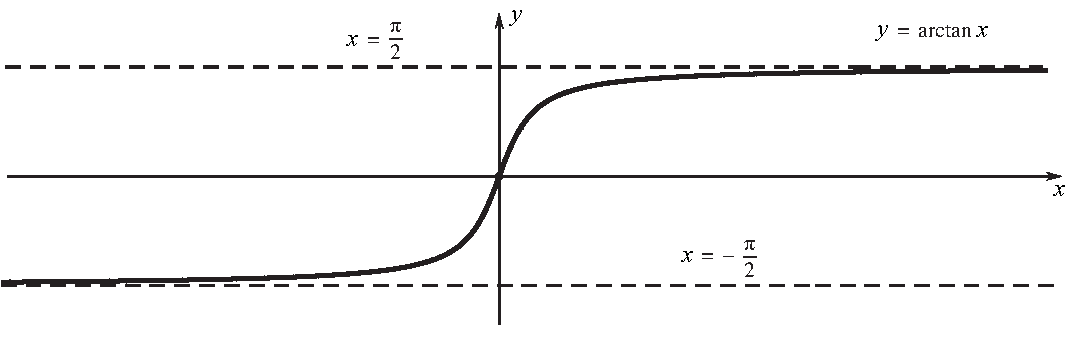
\includegraphics[width = 0.8\linewidth]{pic/C-F/arctan.pdf}
	\vspace*{-1em}
	\caption{$\arctan$函数的图像}
	\label{atan}
\end{figure}
\begin{figure}[!htb]
	\begin{minipage}{0.49\linewidth}
		\centering
		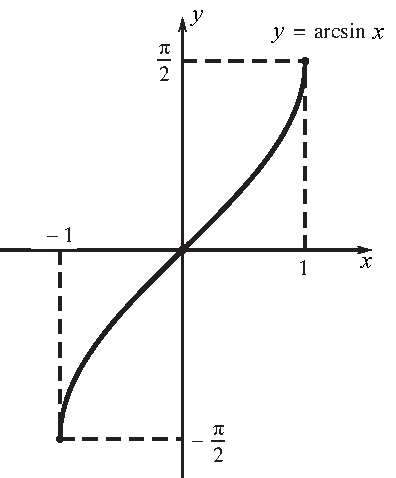
\includegraphics[width=0.89\linewidth]{pic/C-F/arcsin.pdf}
		\caption{$\arcsin$函数的图像}
		\label{asin}
	\end{minipage}
	\begin{minipage}{0.49\linewidth}
		\centering
		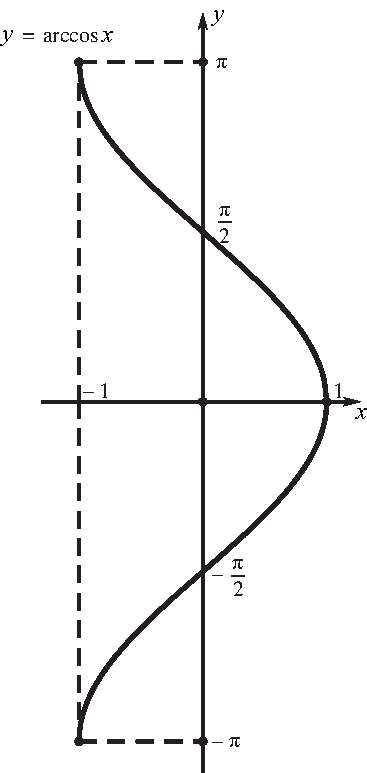
\includegraphics[width=0.51\linewidth]{pic/C-F/arccos.pdf}
		\caption{$\arccos$函数的图像}
		\label{acos}
	\end{minipage}
\end{figure}













